\ifdefined\ishandout
\documentclass[handout]{beamer}
\else
\documentclass{beamer}
\fi

%\usepackage[frenchb]{babel}
\usepackage[T1]{fontenc}
%\usepackage[utf8]{inputenc}
\usepackage{hyperref}
\usepackage{multirow}
\usepackage{listings}
\usepackage{fancyvrb}
\usepackage{tikz}
\usepackage{framed}
\usepackage{algorithm}
\usepackage{algorithmic}
\usepackage{xcolor}
\usepackage{booktabs}
\usepackage{color, colortbl}
\ifdefined\ishandout
\usepackage{handoutWithNotes}
\fi
\usepackage{slashbox}
\usepackage{amsmath}
\usepackage{bm}
\usepackage{hhline}
\usepackage{pgfplots}
\usepackage{caption}
\usepackage{natbib}
\def\bibfont{\footnotesize}
\def\bibname{}


\usetikzlibrary{shapes.geometric}
\usetikzlibrary{positioning}
\usetikzlibrary{shapes.arrows, chains}
\usetikzlibrary{arrows,calc}
\usetikzlibrary{shapes.multipart}
\usetikzlibrary{matrix}

\usepackage{array}
%\usetheme{Boadilla}
\usetheme[progressbar=frametitle]{metropolis}

\usefonttheme[onlymath]{serif}

\newcommand{\R}{\mathbb{R}}
%\newcommand{\C}{\mathbb{C}}
\newcommand{\N}{\mathbb{N}}
\newcommand{\Z}{\mathbb{Z}}
\newcommand{\E}{\mathbb{E}}
\newcommand{\Var}{\text{Var}}
\newcommand{\Cov}{\text{Cov}}
\ifdefined\ishandout
\pgfpagesuselayout{3 on 1 with notes}[a4paper,border shrink=5mm]
\usecolortheme{dove}
\else
%\usecolortheme{dolphin}
%\usecolortheme{crane}
\fi

\metroset{block=fill}

\lstnewenvironment{codeC}
{ \lstset{language=C,
    otherkeywords={printf,scanf}}
}
{}

\ifdefined\ishandout
\definecolor{mygreen}{rgb}{0,0,0}
\definecolor{mymauve}{rgb}{0,0,0}
\definecolor{myblue}{rgb}{0,0,0}
\else
\definecolor{mygreen}{rgb}{0,0.6,0}
\definecolor{mymauve}{rgb}{0.58,0,0.82}
\definecolor{myblue}{rgb}{0,0,1}

\fi

%% Notes
%\setbeameroption{show only notes}


\definecolor{mygray}{rgb}{0.5,0.5,0.5}

\lstset{ language=Python,%
  backgroundcolor=\color{white},   % choose the background color; you must add \usepackage{color} or \usepackage{xcolor}
  basicstyle=\footnotesize,        % the size of the fonts that are used for the code
  breakatwhitespace=false,         % sets if automatic breaks should only happen at whitespace
  breaklines=true,                 % sets automatic line breaking
  captionpos=b,                    % sets the caption-position to bottom
  commentstyle=\color{mygreen},    % comment style
  deletekeywords={...},            % if you want to delete keywords from the given language
  escapeinside={\%*}{*)},          % if you want to add LaTeX within your code
  extendedchars=true,              % lets you use non-ASCII characters; for 8-bits encodings only, does not work with UTF-8
  frame=tb,	                   % adds a frame around the code
  keepspaces=true,                 % keeps spaces in text, useful for keeping indentation of code (possibly needs columns=flexible)
  keywordstyle=\color{blue},       % keyword style
  otherkeywords={*,...},           % if you want to add more keywords to the set
  numbers=none,                    % where to put the line-numbers; possible values are (none, left, right)
  numbersep=5pt,                   % how far the line-numbers are from the code
  numberstyle=\tiny\color{mygray}, % the style that is used for the line-numbers
  rulecolor=\color{black},         % if not set, the frame-color may be changed on line-breaks within not-black text (e.g. comments (green here))
  showspaces=false,                % show spaces everywhere adding particular underscores; it overrides 'showstringspaces'
  showstringspaces=false,          % underline spaces within strings only
  showtabs=false,                  % show tabs within strings adding particular underscores
  stepnumber=2,                    % the step between two line-numbers. If it's 1, each line will be numbered
  stringstyle=\color{mymauve},     % string literal style
  tabsize=3,	                   % sets default tabsize to 2 spaces
  title=\lstname                   % show the filename of files included with \lstinputlisting; also try caption instead of title
}
%\lstset{language=Python,
% breakatwhitespace=false,         % sets if automatic breaks should only happen at whitespace
%  breaklines=true,                 % sets automatic line breaking
%  captionpos=b,                
%%commentstyle=\itshape\color{mymauve},
%%keywordstyle=\bfseries\color{myblue},
%numbers=left,                    % where to put the line-numbers; possible values are (none, left, right)
%  numbersep=8pt,                   % how far the line-numbers are from the code
%  numberstyle=\tiny\color{mygray}, % the style that is used for the line-numbers
%%  rulecolor=\color{black},         % if not set, the frame-color may be changed on line-breaks within not-black text (e.g. comments (green here))
%  showspaces=false,                % show spaces everywhere adding particular underscores; it overrides 'showstringspaces'
%%  showstringspaces=false,          % underline spaces within strings only
%  showtabs=false,                  % show tabs within strings adding particular underscores
%  stepnumber=2,                    % the step between two line-numbers. If it's 1, each line will be numbered
%%  stringstyle=\color{mygreen},     % string literal style
%  tabsize=2 
%}
\ifdefined\ishandout
\newcommand{\red}{\textbf}
\else
\newcommand{\red}{\textcolor{red}}
\fi
%\newcommand \emph
%Default size : 12.8 cm * 9.6 cm

\newcommand{\tmark}[1]{\tikz[remember picture, baseline=-.5ex]{\coordinate(#1);}}

\definecolor{bluegreen}{RGB}{0,149,182}


%\newcommand{\output}[1]{
\setbeamertemplate{navigation symbols}{}
\newcommand{\bvrb}{\Verb[commandchars=£µ§,formatcom=\color{bluegreen}]}
\newcommand{\footvrb}{\footnotesize\Verb}
\newcommand{\vrbalert}[2][]{\visible<#1>{#2}}
%%% Commande pour les listes/arbres
\newcommand{\mvide}{\nodepart{one} \nodepart{two}}
\newcommand{\tvide}{\nodepart{one} \nodepart{two} \nodepart{three}}
\newcommand{\rref}[1][]{\hfill{\scriptsize\textit{#1}}}

%%Fin des commandes pour les listes/arbres.

\bibliographystyle{apalike}

%%% Paramètres du cours (à régler)
%Numéro du cours
\newcommand{\nb}{1}

\title[Machine Learning]{Machine learning and physical modelling-3}
\author[J. Brajard]{julien.brajard@nersc.no}
\institute[NERSC/SU]{NERSC/Sorbonne University\\
\url{https://github.com/brajard/Geilo-Winter-school}}
\date{21-25 January 2018}
\begin{document}
%%%%%%%%%%%%%%%%%%%%% SLIDES DE TITRE
\begin{frame}
\titlepage
%\centering{
%\url{http://australe.upmc.fr} (onglet EPU-C5-IGE Info Gen)}
\end{frame}

\begin{frame}{AI Art?}
    \begin{figure}
        \centering
        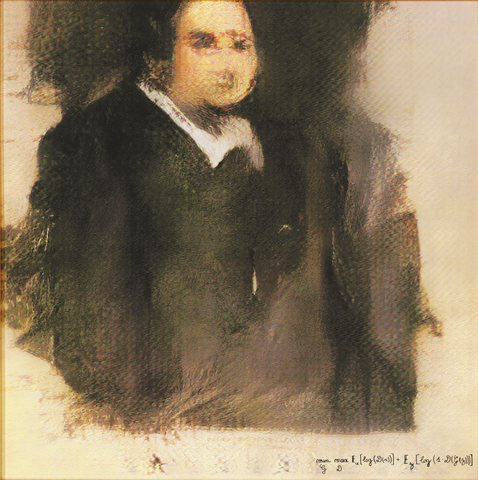
\includegraphics[width=0.5\textwidth]{fig/L3/478px-Edmond_de_Belamy.png}
        \caption*{\textit{Edmond de Bellamy} by Obvious(collective)}
    \end{figure}
    Generated using a Generative Adversarial Network.\\
    Selling prince (Oct. 2018): \$432,000
\end{frame}

\begin{frame}{Table of contents}
  \setbeamertemplate{section in toc}[sections numbered]
  \tableofcontents[hideallsubsections]
\end{frame}

\section{Machine learning to reveal complex connexions}
\begin{frame}{Altimeter data}
\begin{columns}[t]
\column{.5\textwidth}
    \begin{figure}
        \centering
        \caption*{Satellite altimeter}
         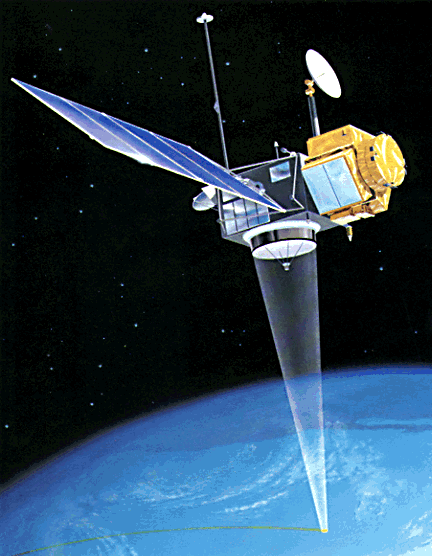
\includegraphics[width=.6\textwidth]{fig/L3/TOPEX-Poseidon.png}
    \end{figure}
    

\column{.5\textwidth}
    \begin{figure}
        \centering
        \caption*{Sea surface height anomaly}
         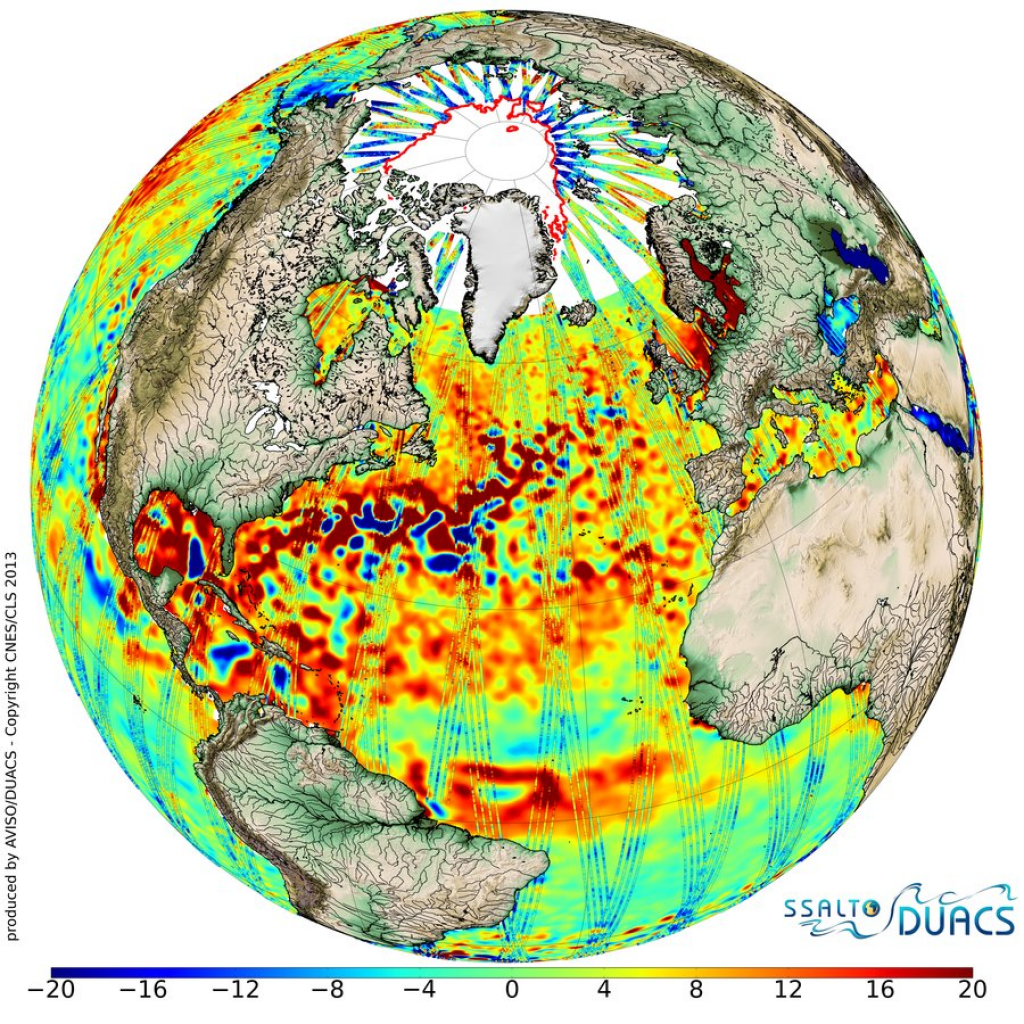
\includegraphics[width=.9\textwidth]{fig/L3/eddies.png}
    \end{figure}

    \end{columns}
    \begin{block}{Structure detection}
    Can we detect and charaterize eddies?
    \end{block}
\end{frame}

\begin{frame}[t]{Eddy detection}
\rref[\cite{Lguensat2017}]
    \begin{columns}
    \column{.65\textwidth}
     \begin{figure}
        \centering
         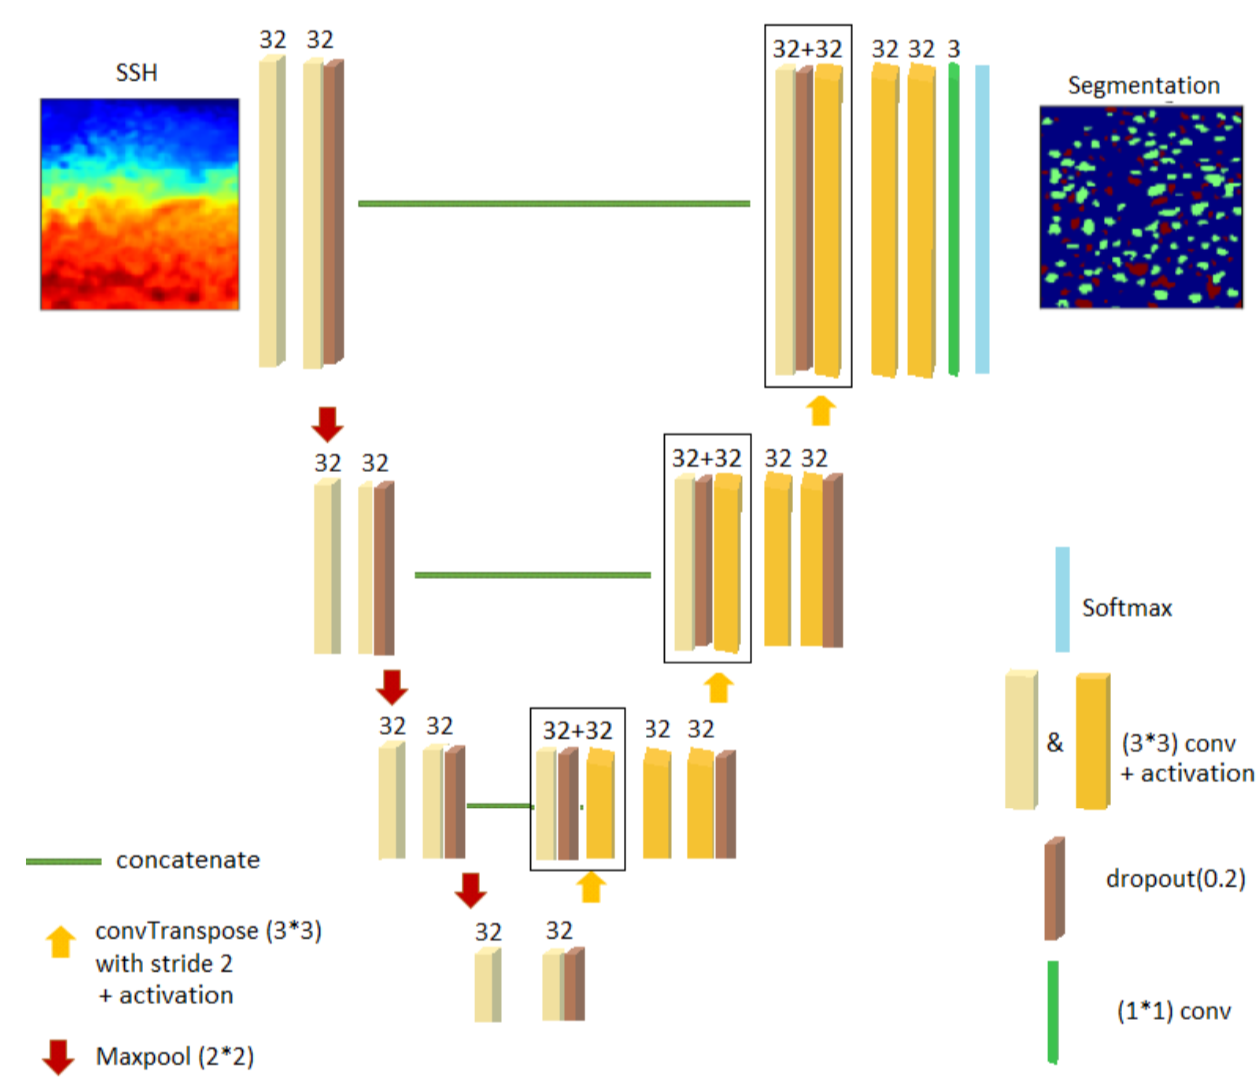
\includegraphics[width=\textwidth]{fig/L3/eddynet.png}
    \end{figure}

    \pause
    \column{.35\textwidth}
         \begin{figure}
        \centering
         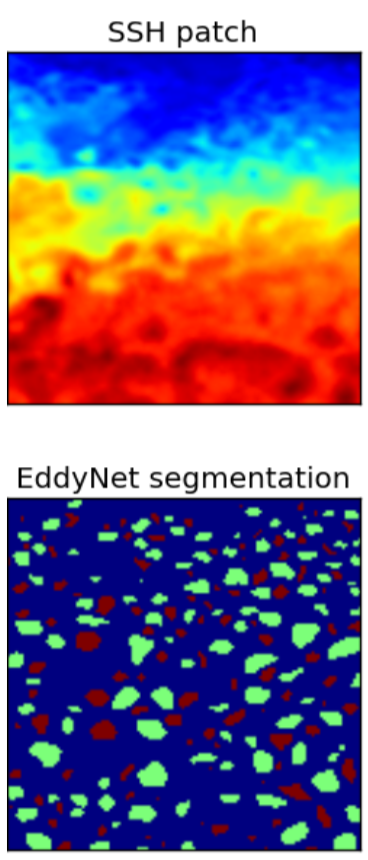
\includegraphics[width=.7\textwidth]{fig/L3/eddynet-result.png}
    \end{figure}
    \end{columns}
\end{frame}

\begin{frame}{Observations of sea velocity}
    %From Sea Surface Height (SSH) it is also possible to derive (partially) the surface currents.
    \begin{columns}
    \column{.4\textwidth}
          \begin{figure}
        \centering
        \caption*{ARGO floats are deployed in the oceans}
         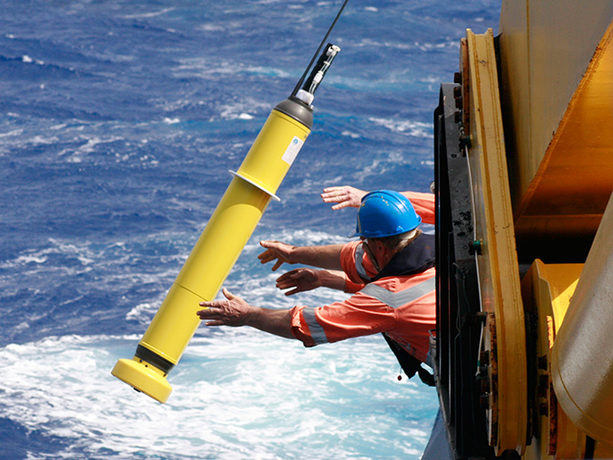
\includegraphics[width=.7\textwidth]{fig/L3/argo-float.jpg}\\
         \end{figure}
         \pause
              \column{.6\textwidth}
\begin{figure}
         \caption*{It measures several \textit{in-situ}  oceanic parameters}
         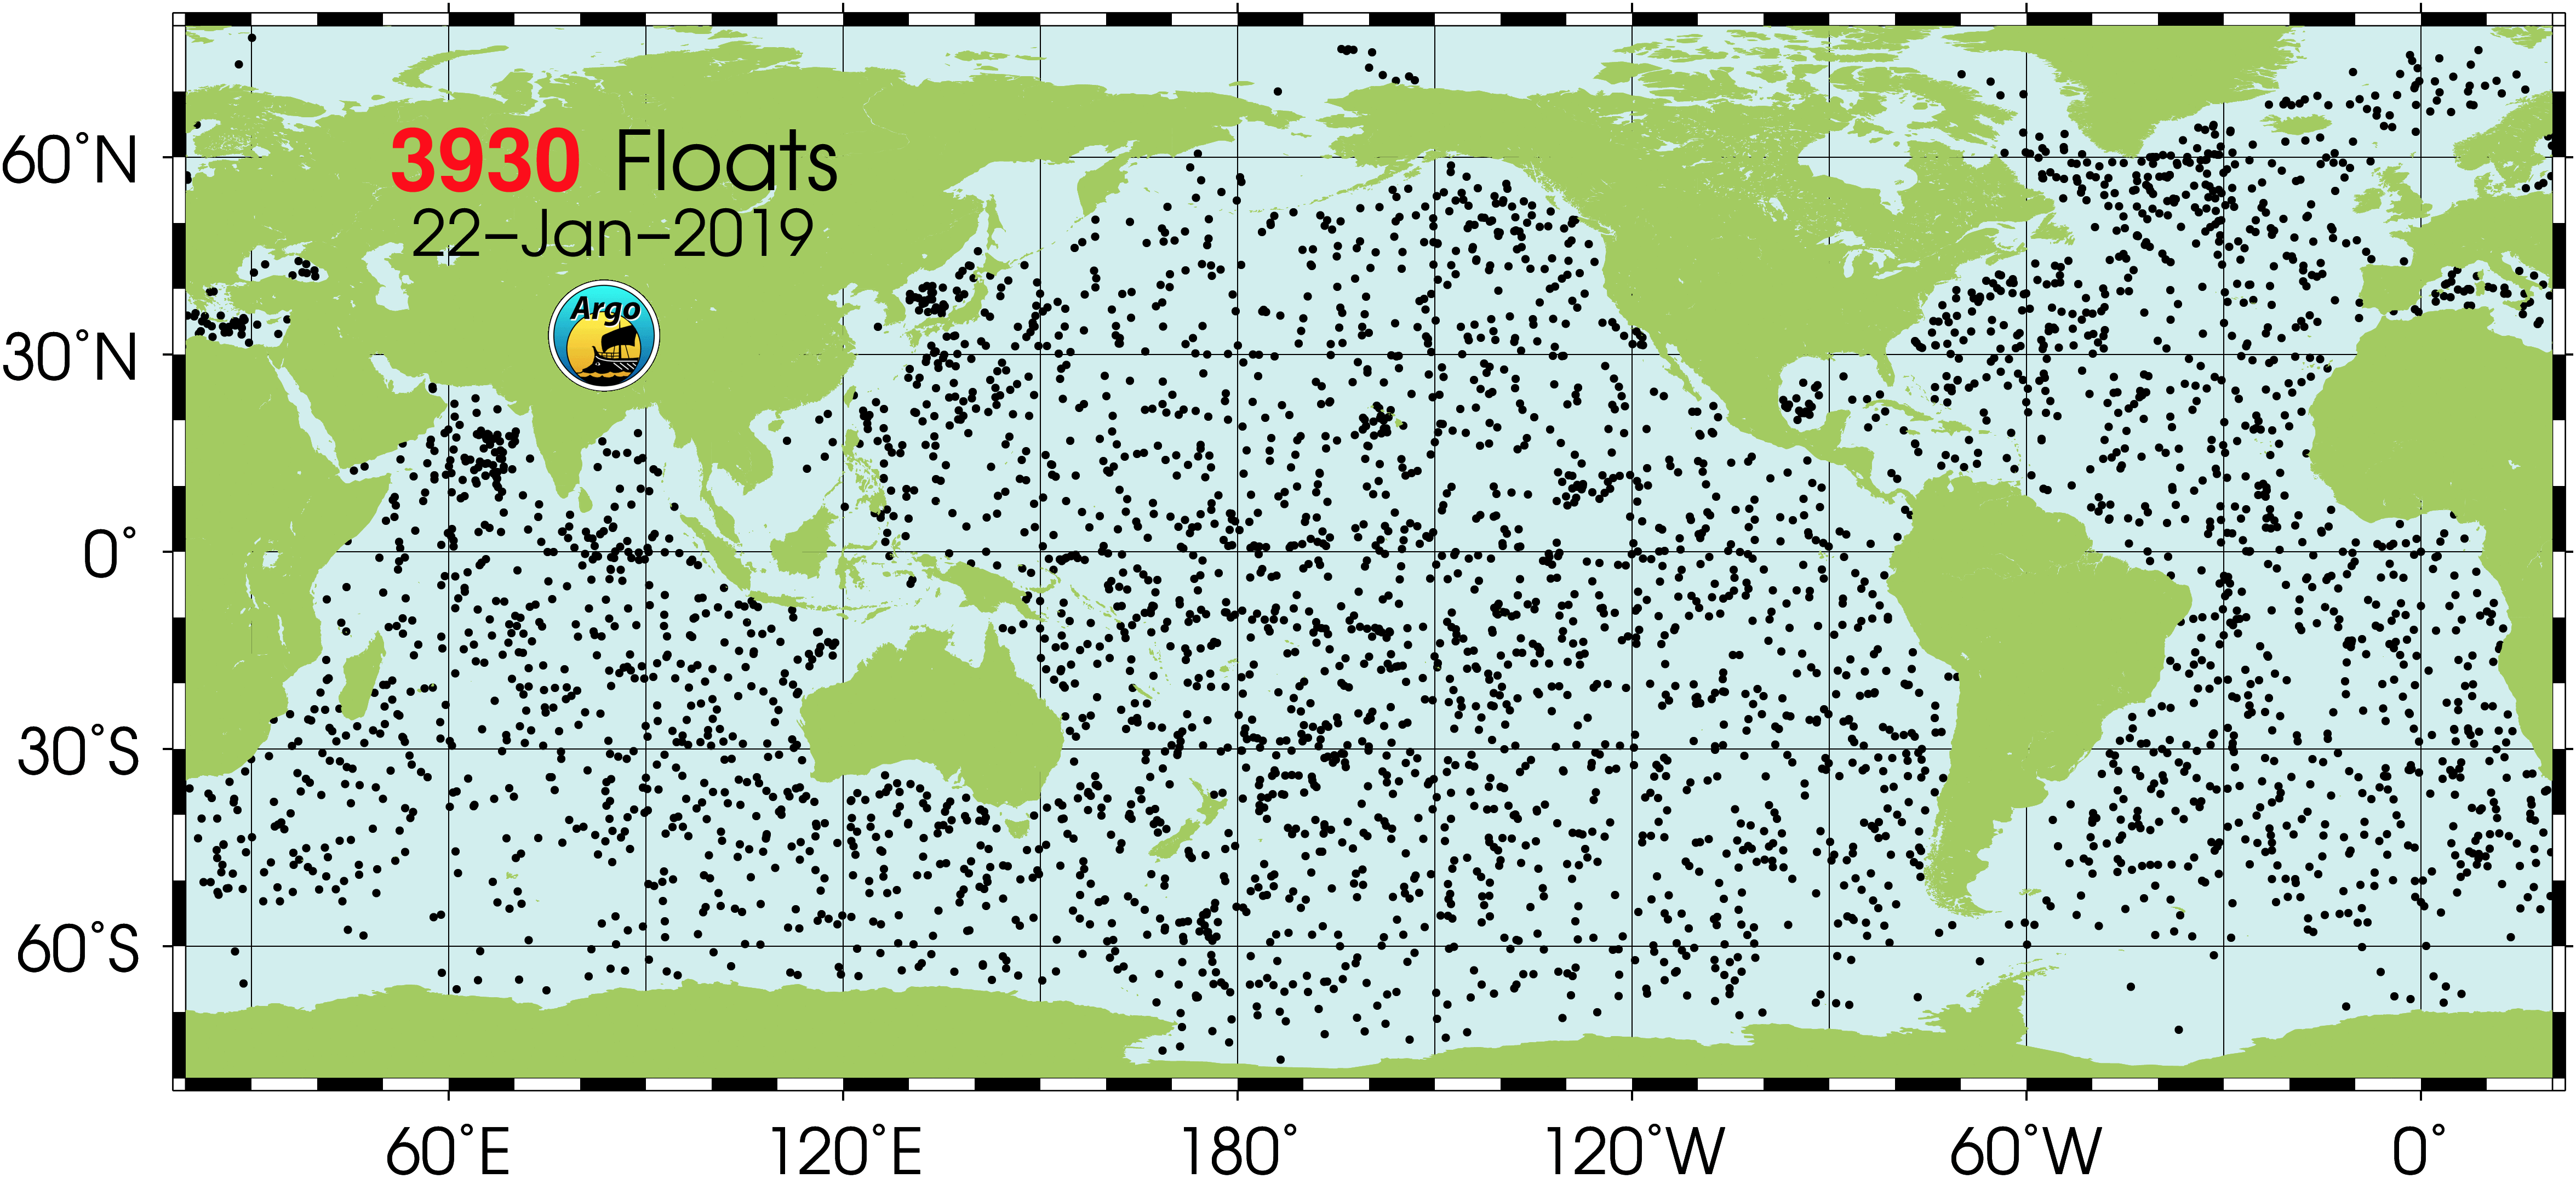
\includegraphics[width=\textwidth]{fig/L3/argo-status.png}
    \end{figure}

    \end{columns}
    
    \begin{columns}
   \pause
    \column{.6\textwidth}
    Matching between:
    \begin{itemize}
        \item Sparse \textit{in-situ} velocity at 1000m
        \item global surface velocity from satellite Sea-Surface heights (SSH).
    \end{itemize}
    \column{.4\textwidth} 
    \begin{figure}
         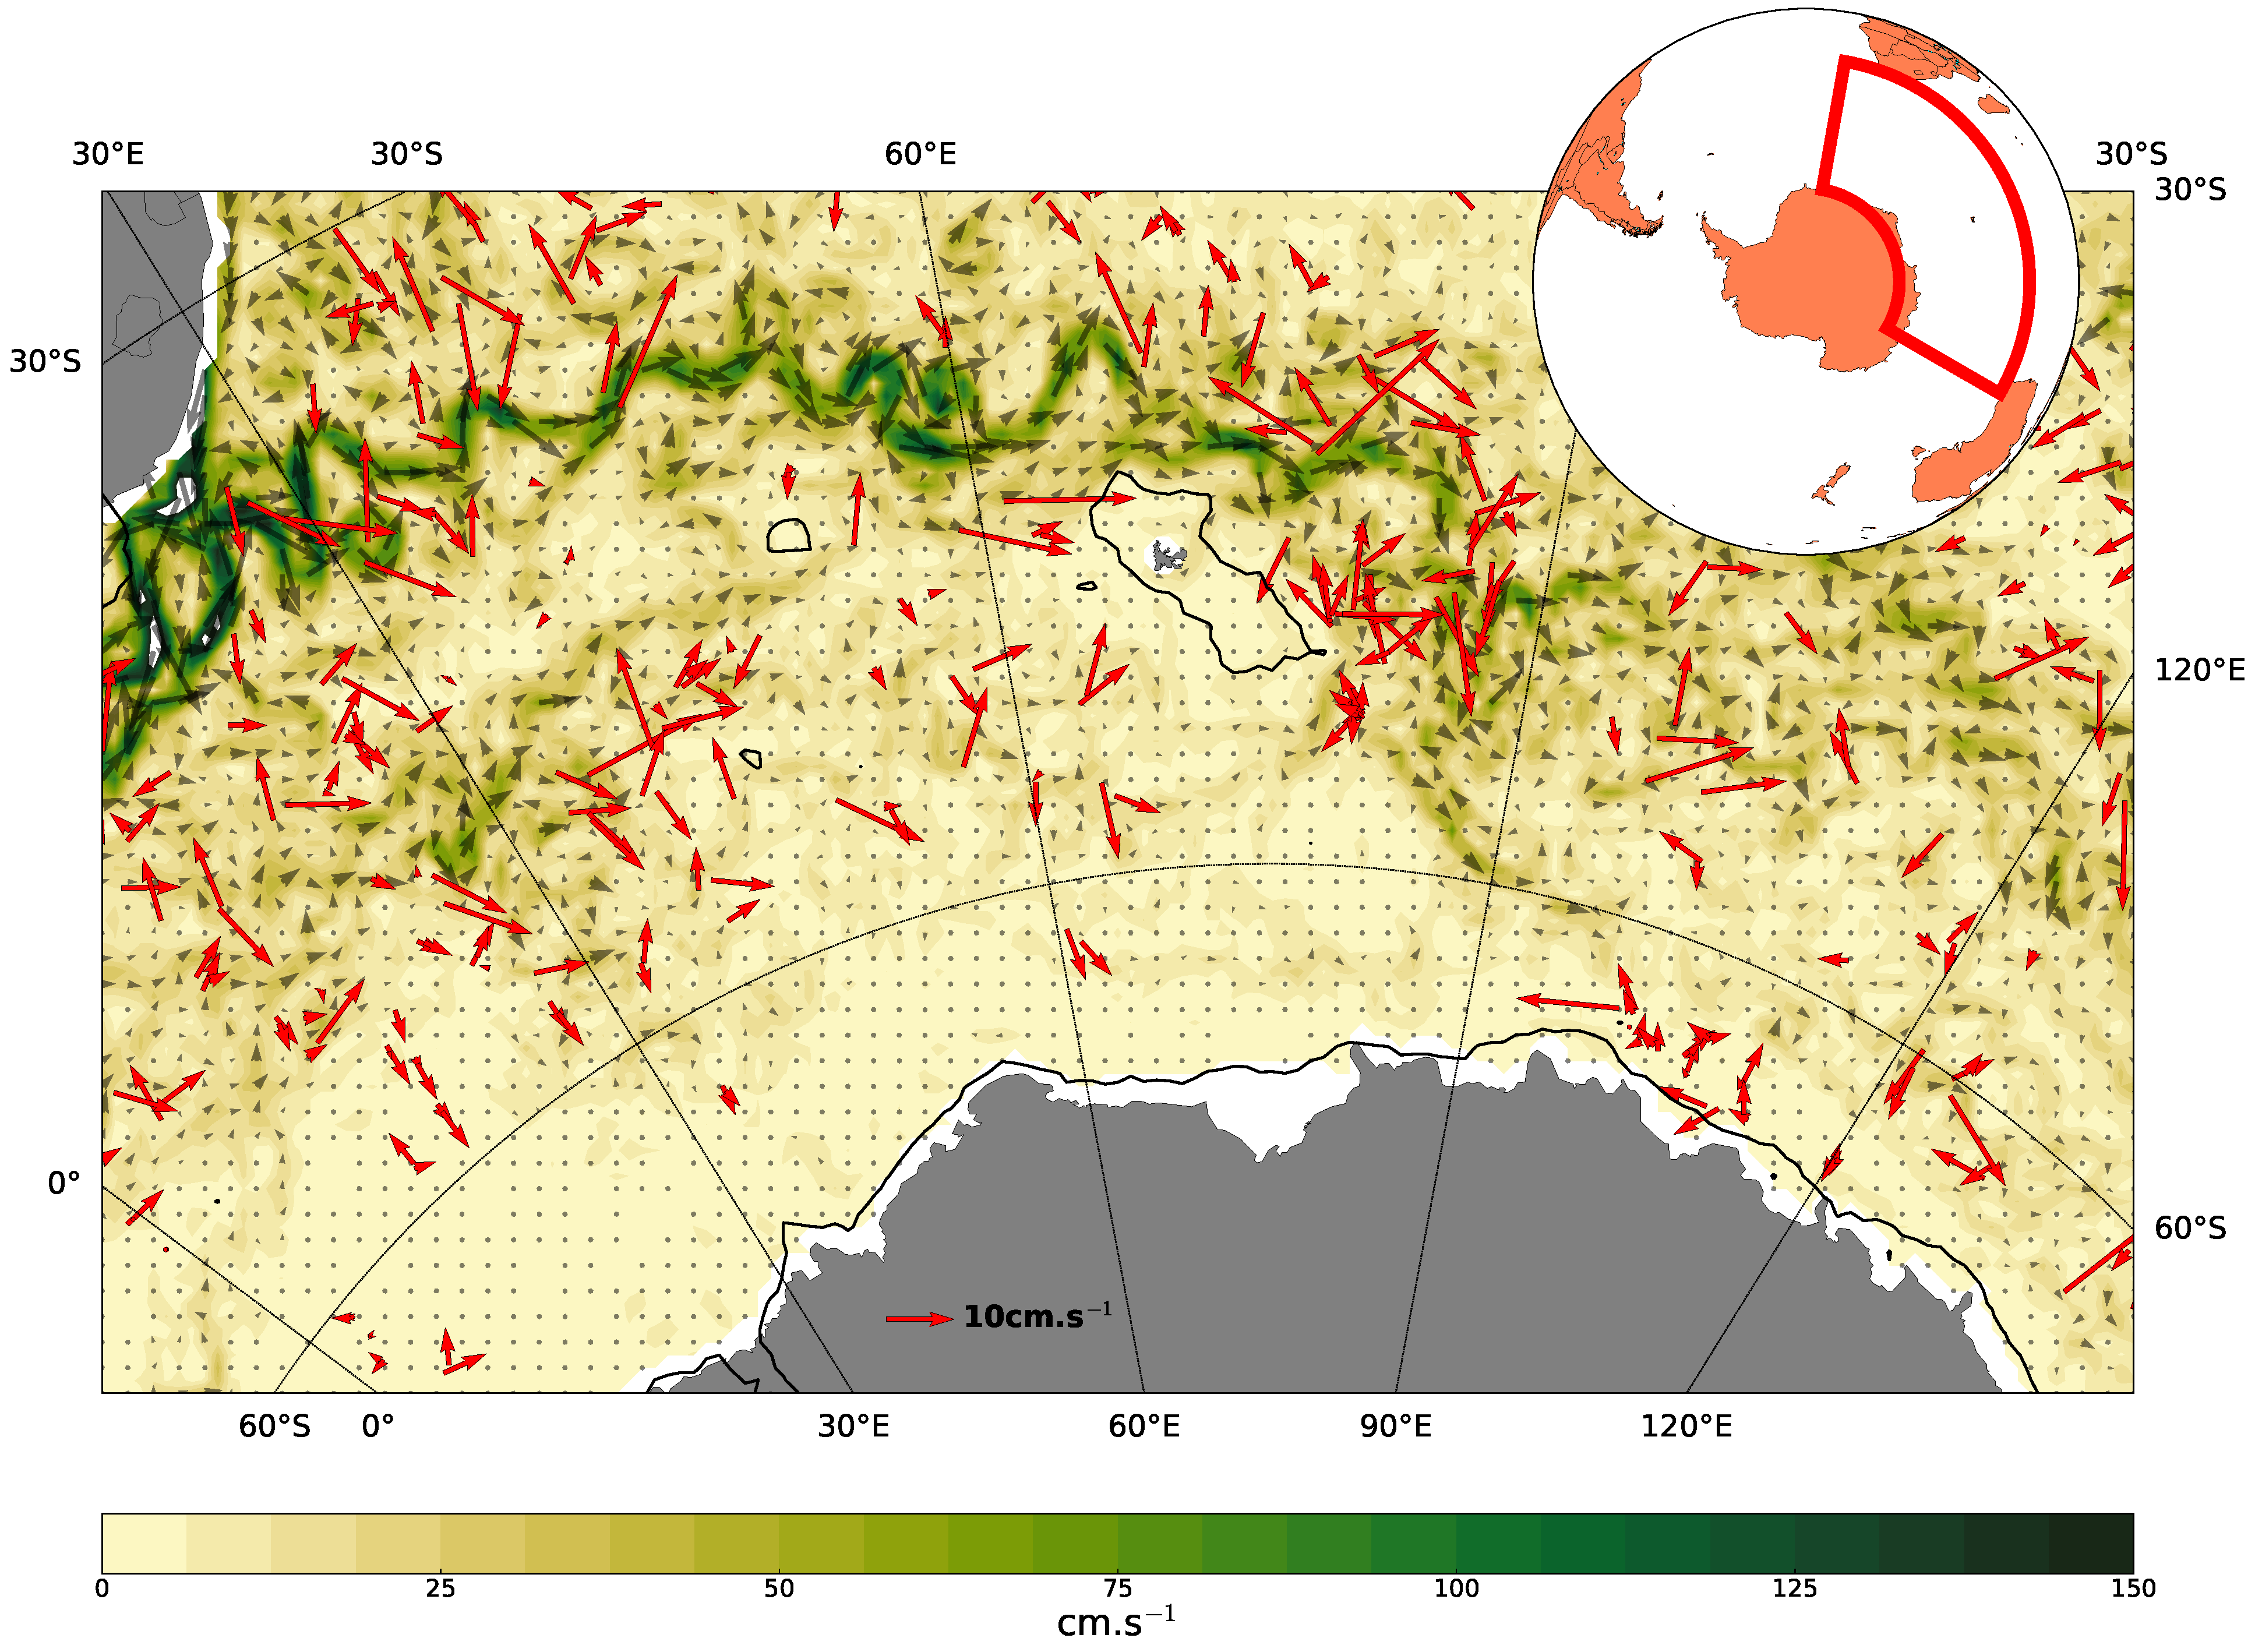
\includegraphics[width=\textwidth]{fig/L3/Surface_Currents_Kerguelen_Intro_resized_v2.pdf}
    \end{figure}
    
    \end{columns}
    \end{frame}
    
    \begin{frame}{Inference of unknown parameters}
        \begin{columns}
        \column{.6\textwidth}
                \rref[\cite{Chapman2017ReconstructionMaps}]

         \begin{figure}
         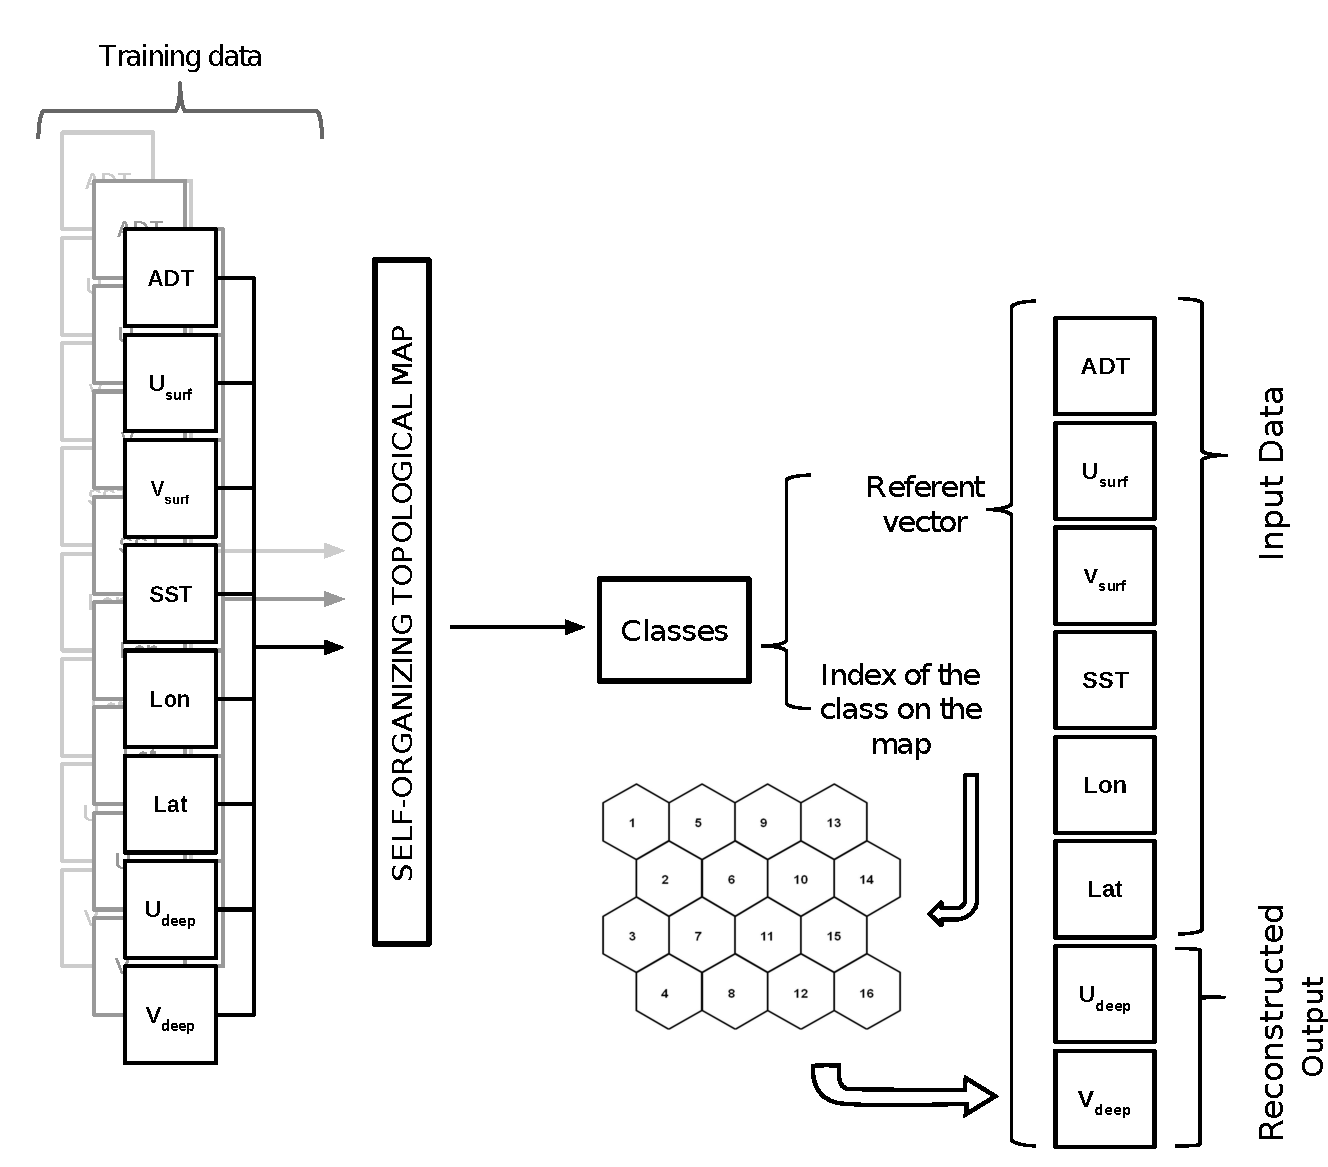
\includegraphics[width=\textwidth]{fig/L3/Method_Schematic_Modified.pdf}
    \end{figure}
    \pause
        \column{.4\textwidth}
         \begin{figure}
         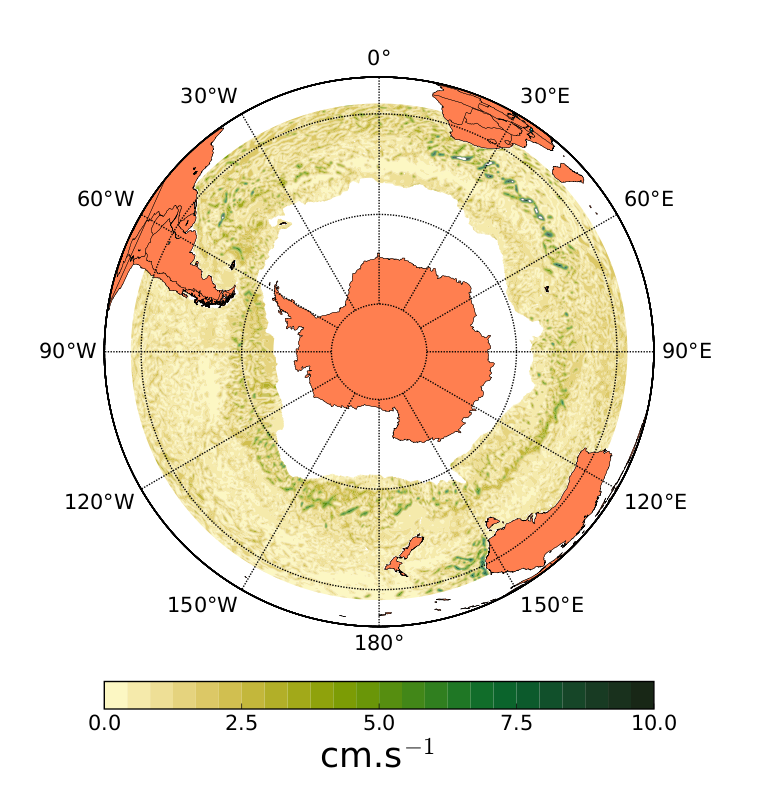
\includegraphics[width=\textwidth]{fig/L3/Deep_Mean_2009_Recon_resized_crop.png}\\
          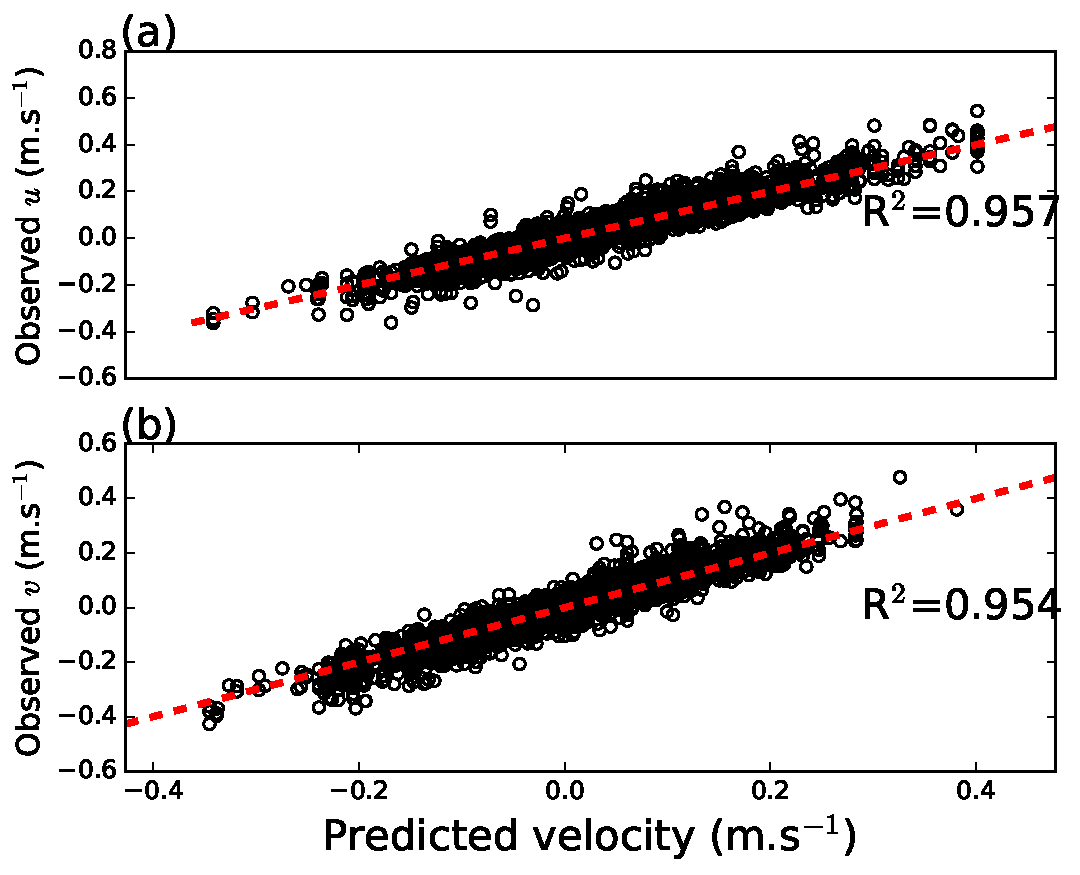
\includegraphics[width=\textwidth]{fig/L3/Scatter_uv_obs_vs_predict_resize.pdf}
    \end{figure}
        \end{columns}
    \end{frame}

\section{Machine learning and differential equations}
\begin{frame}{phyical system and differential equations}
    For example, Motion fluid can be represented using Navier-Stokes equations (PDE):
    
    $$ {\partial{\bf u}\over{\partial t}} = -  ({\bf u} \cdot \nabla) {\bf u} - {1\over\rho} \nabla p + \gamma\nabla^2{\bf u} + {1\over\rho}{\bf F} 
    $$
    \pause
    After spatial discretization, can be represented as an ODE:
    $$
    \frac{d\mathbf{x}}{dt} = f(\mathbf{x(t))}
    $$
\end{frame}

\begin{frame}{ResNET and ODE}
\begin{columns}
\column{.5\textwidth}
Euler discretization scheme:
$$
 x(t+\Delta t) = x + \Delta t.f(x(t)) 
$$
\pause
\column{.5\textwidth}
    \begin{figure}
    \centering
    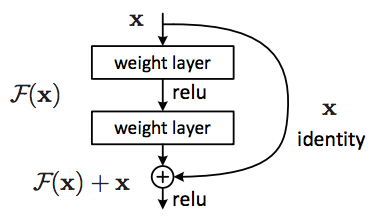
\includegraphics[width=.9\textwidth]{fig/L2/res_block.png}

    \end{figure}
    input: $x(t)$~\\ output:$x(t+\Delta t)$
    $$
    x(t+\Delta t) = x(t) + \Delta t.\mathcal{F}(x(t)) 
    $$
    
    \end{columns}
    \pause
    \alert{Training a ResNet is equivalent to training the underlying model in a Euler discretization scheme}
\end{frame}
\begin{frame}{Other schemes?}
\begin{columns}
\column{.5\textwidth}
\rref[\cite{Fablet2017}]

Runge-Kutta (order 4) integration scheme:
$$
x(t+\Delta t) = x(t) + \sum_{i=1}^4 \alpha_i k_i
$$
where $k_i = f(x(t+\beta_i k_{i-1}\Delta t))$\\
$k_0=0$, 
$\alpha_1=\alpha_4=1/6$,
$\alpha_2=\alpha_3=2/6$,
$\beta_1=\beta_4=1$ 
and  $\beta_2=\beta_3=1/2$.
\pause
\column{.5\textwidth}
\begin{figure}
    \centering
    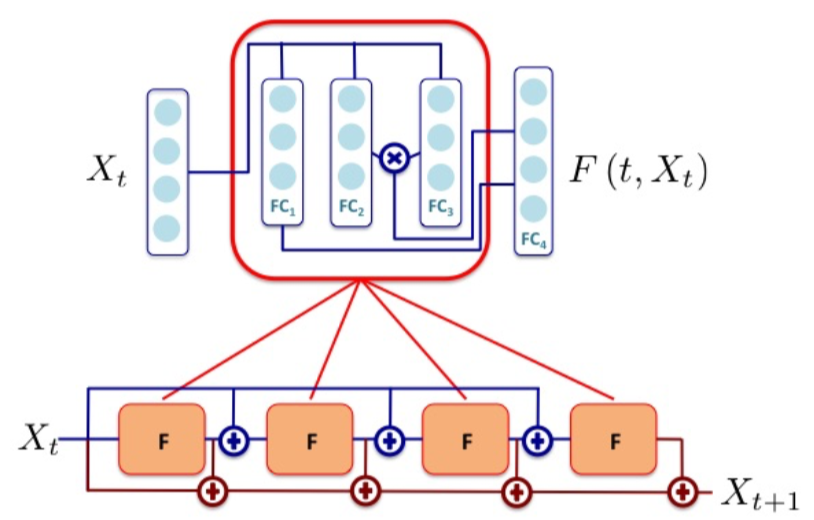
\includegraphics[width=\textwidth]{fig/L3/rk-resnet.png}\\
    \pause
      \caption*{Example on data simulated with a Lorenz 63 system}
     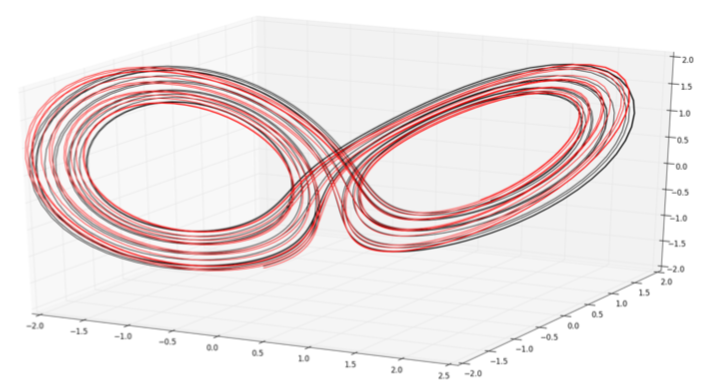
\includegraphics[width=\textwidth]{fig/L3/result-resnet.png}\\
   
\end{figure}
\end{columns}
\end{frame}

\begin{frame}{Toward general framework: Neural ODE}
    \rref[\cite{Chen2018NeuralEquations}: Best paper award NeurIPS, Dec. 2018]
    $$
    \mathbf{z}(t_1) = \mathbf{z}(t_0)  + \int_{t_0}^{t_1} f(\mathbf{z}(t),\theta) dt = \textrm{ODESolve}(\mathbf{z}(t_0),f,t_0,t_1,\theta)
    $$
    \begin{columns}
    \column{.5\textwidth}
    \begin{figure}
        \centering
        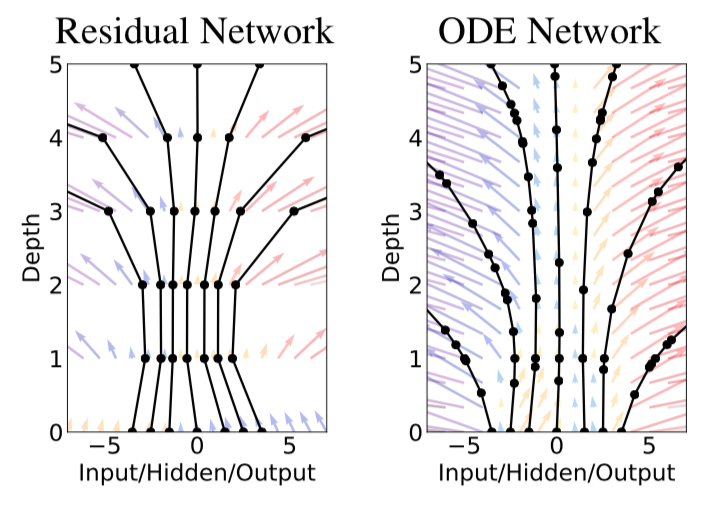
\includegraphics[width=\textwidth]{fig/L3/resVsODE.png}
    \end{figure}
    \column{.5\textwidth}
        \begin{figure}
        \centering
        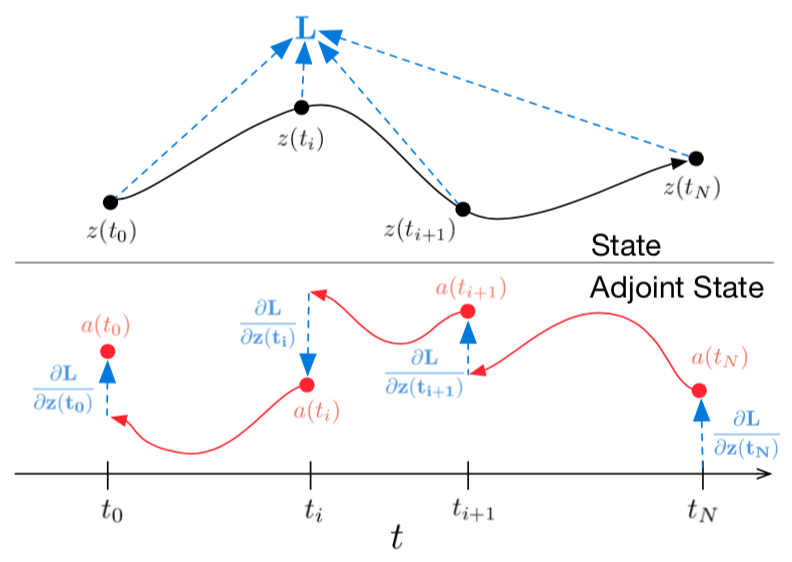
\includegraphics[width=\textwidth,trim={0 5.4cm 0 0},clip]{fig/L3/ODEscheme.png}
    \end{figure}
    \end{columns}
\end{frame}

\begin{frame}{Gradient backpropagation}
\begin{block}{Objective}
Computing $\partial L/ \partial \theta$
\end{block}
 \begin{columns}
   
    \column{.4\textwidth}
        \begin{figure}
        \centering
        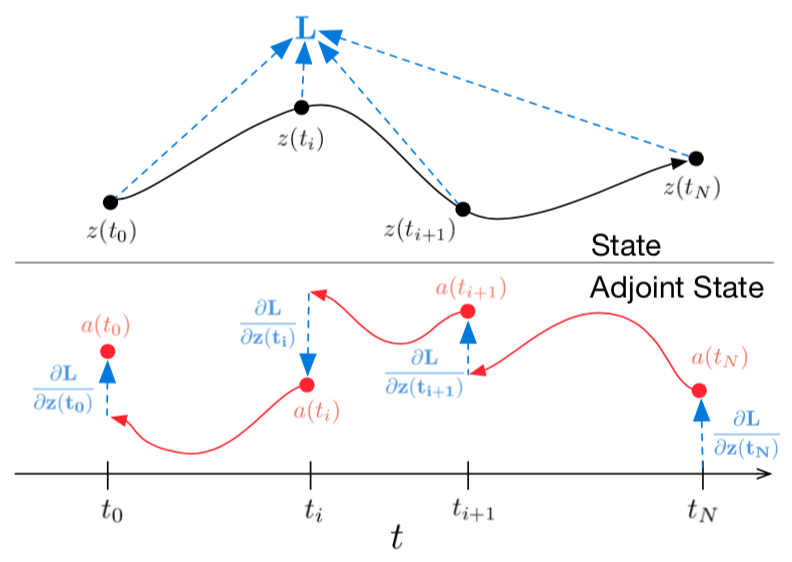
\includegraphics[width=\textwidth]{fig/L3/ODEscheme.png}
    \end{figure}
    \column{.6\textwidth}
    $\mathbf{z}(t_1) = \mathbf{z}(t_0)  + \int_{t_0}^{t_1} f(\mathbf{z}(t),\theta) dt$\\
    Define the adjoint:\\
    $\mathbf{a}(t)=\partial L / d\mathbf{z}(t)$\\
    $$\mathbf{a}(t_0)=\mathbf{a}(t_1) -\int_{t_1}^{t_0} a(t)^T \frac{\partial d f(\mathbf{z(t)},\theta)}{\partial \mathbf{z}}dt$$
      $$\frac{d L}{d\theta}=-\int_{t_1}^{t_0} a(t)^T \frac{\partial d f(\mathbf{z(t)},\theta)}{\partial \theta}dt$$
    
    $a(t)$ and $\frac{d L}{d\theta}=$ can be computed using the Same ODE solver backward in time.
    \end{columns}
\end{frame}

\section{Merge approaches: between physics and machine learning}
\begin{frame}{SST dynamic}
    \rref[\cite{DeBezenac2017TowardsModeling}]
    \begin{block}{Objective}
    Given $SST(t-h),\cdots,SST(t)$, predict $SST(t+\tau)$
    \end{block}
    \begin{figure}
        \centering
        \includegraphics[width=.6\textwidth]{fig/L3/sst}
        \caption{Caption}
        \label{fig:my_label}
    \end{figure}
\end{frame}

\begin{frame}
\begin{figure}
\begin{tikzpicture}
\begin{scope}[text width=8em,anchor=east, align=right]
\node (line2) {Deep learning forecast};
\node [above of = line2,node distance = 1.2cm] (line1) {Reanalysis (truth)};
\node [below of = line2,node distance = 2cm] (line3) {Motion estimate};
\end{scope}
\node [right of = line2, anchor=west, node distance = 1.8cm] (im) {\includegraphics[height=5cm]{./fig/sst.png}};
\end{tikzpicture}
\end{figure}
\end{frame}
\begin{frame}{Shallow-water and the need of additional constraints}
    
\end{frame}

\begin{frame}{}
   \bibliography{references.bib}
\end{frame}
    
%%%%%%%%%%%%%%%%%%%%%
%%%%%%%%%%%%%%%%%%%%%
%%%%%%%%%%%%%%%%%%%%%
%%%%%%%%%%%%%%%%%%%%%
%%%%%%%%%%%%%%%%%%%%%%%%%%%%%%%%%%%%%%%%%%
%%%%%%%%%%%%%%%%%%%%%
%%%%%%%%%%%%%%%%%%%%%%%%%%%%%%%%%%%%%%%%%%
\end{document}
%%%%%%%%%%%%%%%%%%%%%%%%%%%%%%%%%%%%%%%%%%



